\documentclass[aspectratio=169]{beamer}
\usetheme{metropolis}
\metroset{background=dark}
\usepackage[scaled=0.85]{roboto-mono}
\usepackage[english]{babel}
\usepackage[utf8x]{inputenc}
\usepackage[LGR,T1]{fontenc}
\usepackage{listings}
\usepackage{lstautogobble}
\usepackage{selinput}
\usepackage{textalpha}
\usepackage{minted}
\usepackage{caption}
\usepackage{amssymb}
\usepackage[fleqn]{mathtools}
\usepackage[numbers]{natbib}
\usepackage{tikz}
\usepackage{xcolor}
\usepackage{pgfplots}
\usepackage{import}
\usepackage{xspace}
\usepackage{enumerate}
\usepackage{amsmath}
\usepackage{graphicx}
\usepackage{ifthen}
\usepackage{algorithm}
\usepackage{algpseudocode}
\usepackage{algorithmicx}
\usepackage{chngcntr}
\usepackage{tabularx}
\usepackage[sfdefault]{roboto}  %% Option 'sfdefault' only if the base font of the document is to be sans serif
\usepackage{datetime}
\newdate{presentation_date}{27}{06}{2022}

\usetikzlibrary{
    decorations.pathreplacing,
    arrows,
    shapes,
    shapes.gates.logic.US,
    circuits.logic.US,
    calc,
    automata,
    positioning,
    intersections,
    calligraphy,
    tikzmark,
    shadows.blur
}
\setminted{
    xleftmargin=0pt,
    breakanywhere=true,
    breaklines=true,
    linenos=false,
    autogobble,
    style=material,
}

% code listing
\lstdefinestyle{main}{
    numberstyle=\tiny,
    breaklines=true,
    showspaces=false,
    showstringspaces=false,
    tabsize=2,
    numbers=left,
    basicstyle=\ttfamily,
    columns=fixed,
    fontadjust=true,
    basewidth=0.5em,
    autogobble,
    xleftmargin=3.0ex,
    mathescape=true
}

\title{Teaspoon: Parser Combinators in Languages without User-Defined Operators}
\date{\displaydate{presentation_date}}
\author{Eugene Lin}
\institute{Imperial College London}
\begin{document}
    \maketitle
    \begin{frame}{Parser Combinators}
        \onslide<1->
            What even are \textbf<2>{parser} \textbf<4>{combinators}?
        \begin{itemize}
            \itemsep0.75em
            \item<2-> A parser is just a function in \textit{your} favourite programming language!
            \item<3-> Simple functions take an input and obtain a result
            \item<4-> Combinators combine these parsers and create more complex parsers
        \end{itemize}
    \end{frame}
    \section{But why?}
    \begin{frame}[fragile]{Example: Calculator}
        \begin{overprint}
            \onslide<1>
            \begin{minted}{antlr}
                nat  : [0-9]+;
                expr : expr '+' term
                     | expr '-' term
                     | term;
                term : term '*' fact
                     | term '/' fact
                     | fact;
                fact : nat
                     | '(' expr ')';
            \end{minted}
            \onslide<2>
            \begin{minted}{teaspoon_lex.py:TeaspoonLexer -x}
                val  nat  = parseInt <$> /[0-9]+/;
                lazy expr = expr <**> ('+' $> add) <*> term <|>
                            expr <**> ('-' $> sub) <*> term <|>
                            term;
                lazy term = term <**> ('*' $> mul) <*> fact <|>
                            term <**> ('/' $> div) <*> fact <|>
                            fact;
                lazy fact = nat <|>
                            '(' *> expr <* ')';
            \end{minted}
        \end{overprint}
    \end{frame}
    \begin{frame}[fragile]{Example: Arrays and Pairs}
        \begin{overprint}
            \onslide<1>
            \begin{minted}{antlr}
                array  : '[' exprs ']';
                exprs  : exprs ',' expr
                       | expr;
                object : '{' pairs '}';
                pairs  : pairs ',' pair
                       | pair;
            \end{minted}
            \onslide<2>
            \begin{minted}{teaspoon_lex.py:TeaspoonLexer -x}
                val exprs  = expr <:> many(',' *> expr);
                val pairs  = pair <:> many(',' *> pair);
                val array  = '[' *> exprs <* ']';
                val object = '{' *> pairs <* '}';
            \end{minted}
            \onslide<3>
            \begin{minted}[escapeinside=??]{teaspoon_lex.py:TeaspoonLexer -x}
                val exprs  = expr <:> many(',' *> expr);
                val pairs  = pair <:> many(',' *> pair);?\tikzmark{marker}?
                val array  = '[' *> exprs <* ']';
                val object = '{' *> pairs <* '}';
            \end{minted}
            \tikz[remember picture] {
                \node[overlay, materialRed600] (comment) at (9, 0) {\shortstack{-10,000 too much\\code duplication}};
                \draw[overlay, materialRed600] (comment) edge[thick, ->, bend right=50] ($(pic cs:marker) + (0, 0.33)$);
            }
            \onslide<4>
            \begin{minted}{teaspoon_lex.py:TeaspoonLexer -x}
                function commaSep<A>(p: Parser<A>): Parser<A[]> {
                    return p <:> many(',' *> p);
                }
                val array  = '[' *> commaSep(expr) <* ']';
                val object = '{' *> commaSep(pair) <* '}';
            \end{minted}
        \end{overprint}
    \end{frame}
    \begin{frame}{Why Parser Combinators?}
        \onslide<1->
            How are they better than parser generators?
        \begin{itemize}
            \itemsep0.75em
            \item<2-> Easily obtain the desired result
            \item<3-> Lexing, parsing, and building AST in a single pass
            \item<4-> Host abstraction: \emph{you} can build anything that's missing!
            \item<5-> Parser combinators embody software engineering principles
        \end{itemize}
    \end{frame}
    \section{Demo}
    \section{Something's wrong...}
    \begin{frame}[fragile]{Left Recursion}
        \begin{overprint}
            \begin{minted}{teaspoon_lex.py:TeaspoonLexer -x}
                val  nat  = parseInt <$> /[0-9]+/;
                lazy expr = expr <**> ('+' $> add) <*> term <|>
                            expr <**> ('-' $> sub) <*> term <|>
                            term;
                lazy term = term <**> ('*' $> mul) <*> fact <|>
                            term <**> ('/' $> div) <*> fact <|>
                            fact;
                lazy fact = nat <|>
                            '(' *> expr <* ')';
            \end{minted}
        \end{overprint}
    \end{frame}
    \begin{frame}[plain]{A Real Problem}
        \vspace{-0.25\baselineskip}
        \hspace*{-2cm}
        \begin{tikzpicture}
            \onslide<1->\node[rotate=0, blur shadow={shadow blur steps=20, shadow xshift=0pt, shadow yshift=0pt, shadow blur radius=10pt, shadow scale=0.95}] at (0, 0) {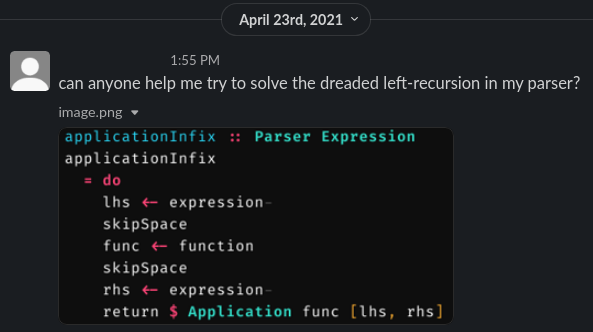
\includegraphics[width=0.75\linewidth]{img/slack_wg.png}};
            \onslide<2->\node[rotate=10, blur shadow={shadow blur steps=20, shadow xshift=0pt, shadow yshift=0pt, shadow blur radius=10pt, shadow scale=0.95}] at (0, 2) {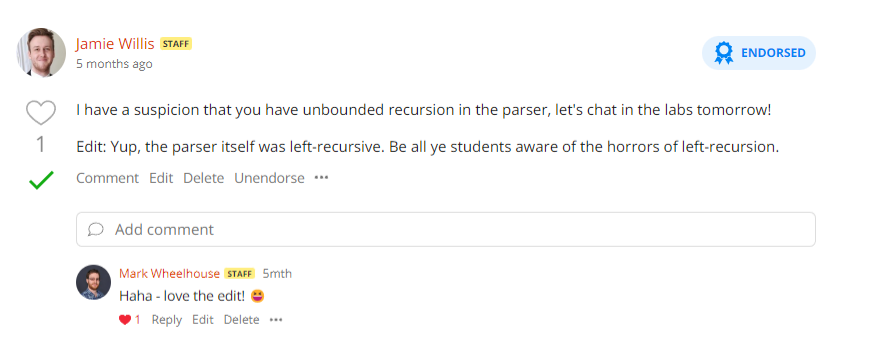
\includegraphics[width=0.75\linewidth]{img/edstem0.png}};
            \onslide<3->\node[rotate=-14, blur shadow={shadow blur steps=20, shadow xshift=0pt, shadow yshift=0pt, shadow blur radius=10pt, shadow scale=0.95}] at (4, 1) {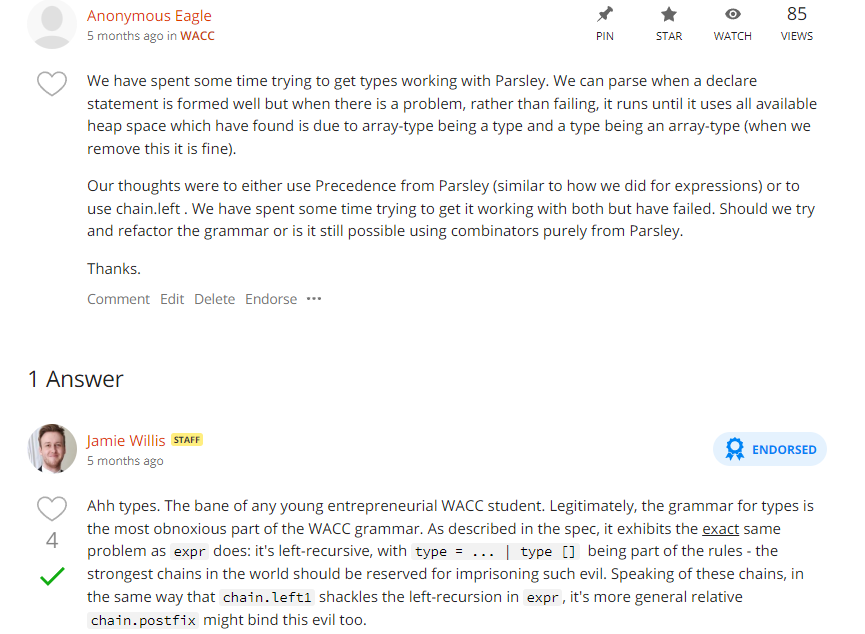
\includegraphics[width=0.75\linewidth]{img/edstem1.png}};
            \onslide<4->\node[rotate=24, blur shadow={shadow blur steps=20, shadow xshift=0pt, shadow yshift=0pt, shadow blur radius=10pt, shadow scale=0.95}] at (-2.1, 1.4) {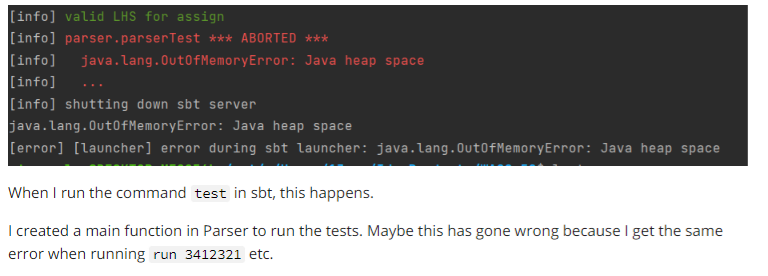
\includegraphics[width=0.75\linewidth]{img/edstem2.png}};
            \onslide<5->\node[rotate=5, blur shadow={shadow blur steps=20, shadow xshift=0pt, shadow yshift=0pt, shadow blur radius=10pt, shadow scale=0.95}] at (-1, 4.5) {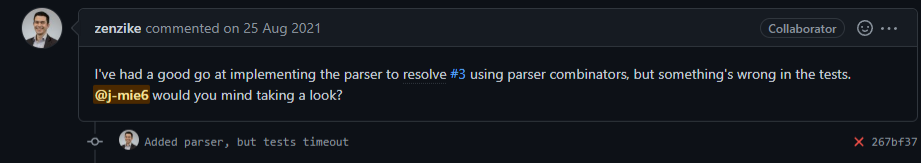
\includegraphics[width=0.75\linewidth]{img/nick0.png}};
            \onslide<6->\node[rotate=-3, blur shadow={shadow blur steps=20, shadow xshift=0pt, shadow yshift=0pt, shadow blur radius=10pt, shadow scale=0.95}] at (-0.5, -1.5) {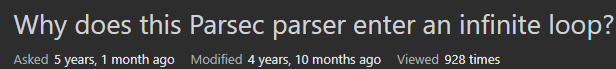
\includegraphics[width=0.75\linewidth]{img/so0.png}};
            \onslide<7->\node[rotate=-10, blur shadow={shadow blur steps=20, shadow xshift=0pt, shadow yshift=0pt, shadow blur radius=10pt, shadow scale=0.95}] at (2.5, 0.75) {
\includegraphics[width=0.85\linewidth]{img/nick1.png}};
        \end{tikzpicture}
    \end{frame}
    \begin{frame}[fragile]{Chains}
        \begin{overprint}
            \onslide<1>
            \begin{minted}{teaspoon_lex.py:TeaspoonLexer -x}
                val  nat  = parseInt <$> /[0-9]+/;
                lazy expr = expr <**> ('+' $> add) <*> term <|>
                            expr <**> ('-' $> sub) <*> term <|>
                            term;
                lazy term = term <**> ('*' $> mul) <*> fact <|>
                            term <**> ('/' $> div) <*> fact <|>
                            fact;
                lazy fact = nat <|>
                            '(' *> expr <* ')';
            \end{minted}
            \onslide<2>
            \begin{minted}{teaspoon_lex.py:TeaspoonLexer -x}
                val  nat  = parseInt <$> /[0-9]+/;
                lazy expr = chainl1(term,
                    ('+' $> add) <|> ('-' $> sub)
                );
                lazy term = chainl1(fact,
                    ('*' $> mul) <|> ('/' $> div)
                );
                lazy fact = nat <|>
                            '(' *> expr <* ')';
            \end{minted}
        \end{overprint}
    \end{frame}
    \section{Demo}
    \section{The Preprocessor}
    \begin{frame}[fragile]{Pipeline}
        \begin{overprint}
            \onslide<1>
            \begin{center}
                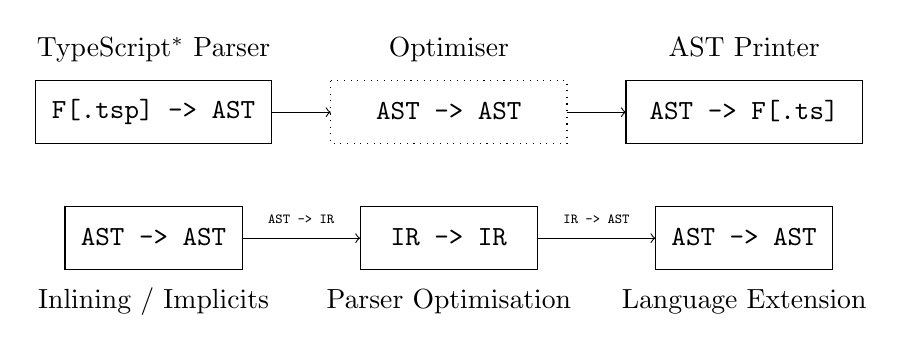
\begin{tikzpicture}[every node/.style={execute at end node=\vphantom{bg}},x=0.75cm, y=0.8cm]
                    \begin{scope}[shift={(0, 0)}]
                        \node at (0, 0) {\texttt{F[.tsp] -> AST}};
                        \node at (0, 1) {TypeScript$^*$ Parser};
                        \draw (-2, 0.5) -- (2, 0.5) -- (2, -0.5) -- (-2, -0.5) -- cycle;
                    \end{scope}
                    \begin{scope}[shift={(5, 0)}]
                        \node at (0, 0) {\texttt{AST -> AST}};
                        \node at (0, 1) {Optimiser};
                        \draw[dotted] (-2, 0.5) -- (2, 0.5) -- (2, -0.5) -- (-2, -0.5) -- cycle;
                    \end{scope}
                    \begin{scope}[shift={(10, 0)}]
                        \node at (0, 0) {\texttt{AST -> F[.ts]}};
                        \node at (0, 1) {AST Printer};
                        \draw (-2, 0.5) -- (2, 0.5) -- (2, -0.5) -- (-2, -0.5) -- cycle;
                    \end{scope}
                    \begin{scope}[shift={(0, -2)}]
                        \node at (0, 0) {\texttt{AST -> AST}};
                        \node at (0, -1) {Inlining / Implicits};
                        \draw (-1.5, 0.5) -- (1.5, 0.5) -- (1.5, -0.5) -- (-1.5, -0.5) -- cycle;
                    \end{scope}
                    \begin{scope}[shift={(5, -2)}]
                        \node at (0, 0) {\texttt{IR -> IR}};
                        \node at (0, -1) {Parser Optimisation};
                        \draw (-1.5, 0.5) -- (1.5, 0.5) -- (1.5, -0.5) -- (-1.5, -0.5) -- cycle;
                    \end{scope}
                    \begin{scope}[shift={(10, -2)}]
                        \node at (0, 0) {\texttt{AST -> AST}};
                        \node at (0, -1) {Language Extension};
                        \draw (-1.5, 0.5) -- (1.5, 0.5) -- (1.5, -0.5) -- (-1.5, -0.5) -- cycle;
                    \end{scope}
                    \draw
                    (2, 0) edge[->] (3, 0)
                    (7, 0) edge[->] (8, 0)
                    % (4, -0.5) edge[->] (-0.5, -1.5)
                    % (10.5, -1.5) edge[->] (6, -0.5)
                    (1.5, -2) edge[->, above] node{\tiny \texttt{AST -> IR}} (3.5, -2)
                    (6.5, -2) edge[->, above] node{\tiny \texttt{IR -> AST}} (8.5, -2);

                    \draw[pen colour={white}, very thick, decorate, decoration={calligraphic brace, amplitude=5pt, raise=-2pt}] (-1.5, -1) -- (11.5, -1);
                \end{tikzpicture}
            \end{center}
        \end{overprint}
    \end{frame}
    \begin{frame}[fragile]{Extending TypeScript}
        \onslide<1->
            Main differences from TypeScript:
        \begin{itemize}
            \itemsep0.75em
            \item<2-> \textbf<2-3>{New declarations and laziness}
            \item<4-> \textbf<4-5>{User-defined operators}
            \item<6-> \textbf<6-7>{`Macros'}
        \end{itemize}
        \bigskip

        \begin{overprint}
            \onslide<2>
            \begin{minted}{teaspoon_lex.py:TeaspoonLexer -x}
                lazy p = p;
                val q = x;
            \end{minted}
            \onslide<3>
            \begin{minted}{typescript}
                const p = lazy(() => p);
                const q = x;
            \end{minted}
            \onslide<4>
            \begin{minted}{teaspoon_lex_with_cust_op.py:TeaspoonLexer -x}
                let p = a <~> b;
                let q = a *> b *> c;
                let r = a <*> b <|> c <*> d;
                let s = a <**> (pf <* b) <*> c;
                let t = a <xyz> b;
            \end{minted}
            \onslide<5>
            \begin{minted}{typescript}
                let p = mult(q, r);
                let q = apR(apR(a, b), c);
                let r = choice(ap(a, b), ap(c, d));
                let s = ap(pa(a, apL(pf, b)), c);
                let t = xyz(a, b);
            \end{minted}
            \onslide<6>
            \begin{minted}{teaspoon_lex.py:TeaspoonLexer -x}
                inline paap(x, y, z) = x <**> y <*> z;
                inline o = add <$ chr('+');
                inline add = (x: number) => (y: number) => x + y;
                let r = paap(a, o, b);
            \end{minted}
            \onslide<7>
            \begin{minted}{typescript}
                let r = ap(pa(a,
                  constFmapL(
                    (x: number) => (y: number) => x + y,
                    chr('+')
                )), b);
            \end{minted}
        \end{overprint}
    \end{frame}
    \begin{frame}[fragile]{Removing Left Recursion}
        \begin{overprint}
            \onslide<1>
            \begin{minted}{teaspoon_lex.py:TeaspoonLexer -x}
                val nat   = parseInt <$> /[0-9]+/;
                lazy expr = (x => y => x + y) <$> (expr <* '+') <*> nat <|>
                            expr <**> ((x => y => x - y) <$ '-') <*> nat <|>
                            nat;
            \end{minted}
            \onslide<2>
            \begin{minted}{typescript}
                const nat  = fmap(parseInt, re(/[0-9]+/));
                const expr = lazy(() => postfix(nat,
                    choice(
                        pamf(apR(chr('-'), nat), (y) => (x) => x - y),
                        pamf(apR(chr('+'), nat), (y) => (x) => x + y)
                    )
                ));
            \end{minted}
        \end{overprint}
    \end{frame}
    \begin{frame}[fragile]{Rewriting}
        \onslide<1->
            Rewriting is done in three steps:
        \begin{enumerate}
            \itemsep0.75em
            \item<2-> \textbf<2-3>{Normalisation}
            \item<4-> \textbf<4>{Reduction}
            \item<5-> \textbf<5-6>{Postfix rewrite}
        \end{enumerate}
        \bigskip

        \begin{overprint}
            \onslide<2>
            \begin{minted}{teaspoon_lex.py:TeaspoonLexer -x}
                lazy e = (x => y => x + y) <$> (e <* '+') <*> n <|> n;
            \end{minted}
            \onslide<3>
            \begin{minted}{teaspoon_lex.py:TeaspoonLexer -x}
                lazy e = lift2(u(x => y => x + y), e <* '+', n) <|> n;
            \end{minted}
            \onslide<4>
            \begin{minted}{teaspoon_lex_with_cust_op.py:TeaspoonLexer -x}
                lazy e = lift2(u(x => y => x + y), e, '+' *> n) <|> n;
            \end{minted}
            \onslide<5>
            \begin{minted}{teaspoon_lex_with_cust_op.py:TeaspoonLexer -x}
                lazy e = postfix(n,
                    f(c(u(x => y => x + y))) <$> ('+' *> n)
                );
            \end{minted}
            \onslide<6>
            \begin{minted}{teaspoon_lex_with_cust_op.py:TeaspoonLexer -x}
                lazy e = postfix(n,
                    (y => x => x + y) <$> ('+' *> n)
                );
            \end{minted}
        \end{overprint}
    \end{frame}
    \section{Conclusion}
    \begin{frame}{Contributions}
        \onslide<1->
            Contributions:
        \begin{itemize}
            \itemsep0.75em
            \item<2-> A lightweight parser combinator library for TypeScript
            \item<3-> A pipeline for analysing and extending TypeScript
            \item<4-> Techniques for detecting and refactoring left-recursion and general parser optimisations such as backtracking removal
                \onslide<5->
                \begin{itemize}
                    \item Correctness of these transformations have been reasoned about in the report
                \end{itemize}
        \end{itemize}
    \end{frame}
    \begin{frame}{Related Works}
        \onslide<1->
            This isn't a new problem:
        \begin{itemize}
            \itemsep0.75em
            \item<2-> \textit{ANTLR4}: a parser generator that rewrites left-recursion
            \item<3-> Other TypeScript parser combinator libraries (\textit{ts-parsec}, \textit{parsimmon})
            \item<4-> Baars \& Swierstra's self inspecting parsers
        \end{itemize}
    \end{frame}
    \begin{frame}{Thanks for Listening!}
        \onslide<1->
            What have we seen?
        \begin{itemize}
            \itemsep0.75em
            \item<2-> Parser combinators are an effective way of performing real parsing
            \item<3-> TypeScript doesn't support it well
            \item<4-> Left-recursion is a real problem that complicates parser combinators
            \item<5-> These problems, and more, can be solved with a preprocessor
        \end{itemize}
    \end{frame}
\end{document}